
\newpage

\section{Вариант 2}

Дополнительные настройки для компьютера 3:

\begin{verbatim}
iptables  -t mangle -F
ip6tables -t mangle -F

iptables  -t mangle -I PREROUTING -p tcp -d        5.6.12.2 -j MARK --set-mark 2
ip6tables -t mangle -I PREROUTING -p tcp -d ::ffff:5.6.12.2 -j MARK --set-mark 2

ip    rule a from all fwmark 2 lookup netcat2
ip -6 rule a from all fwmark 2 lookup netcat2

ip    r a default via        5.6.13.1 dev enp0s8 table netcat2
ip -6 r a default via ::ffff:5.6.13.1 dev enp0s8 table netcat2
\end{verbatim}

\subsection{Скриншоты выполнения}

Передадим сообщения
\begin{itemize}
    \item \texttt{Client -> Server 1} --- от клиента 1 к серверу 1
    \item \texttt{Server -> Client 1} --- от сервера 1 к клиенту 1
    \item \texttt{Client -> Server 2} --- от клиента 2 к серверу 2
    \item \texttt{Server -> Client 2} --- от сервера 2 к клиенту 2
\end{itemize}

\subsubsection{Сервер 1}
\paragraph{IPv4}
\begin{center}
    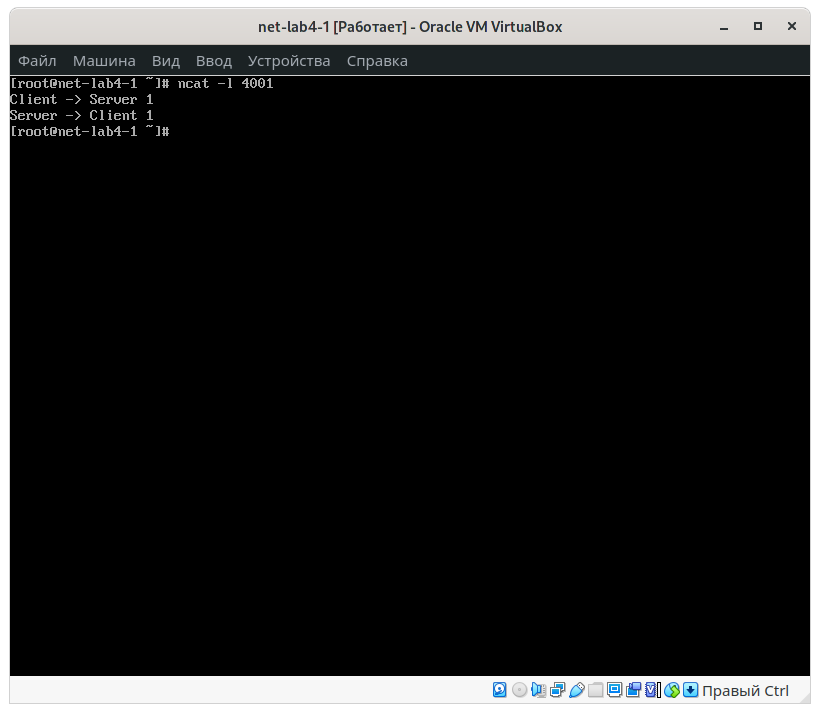
\includegraphics[width=.49\textwidth]{screenshots/var2-ncat1-server-ipv4}
    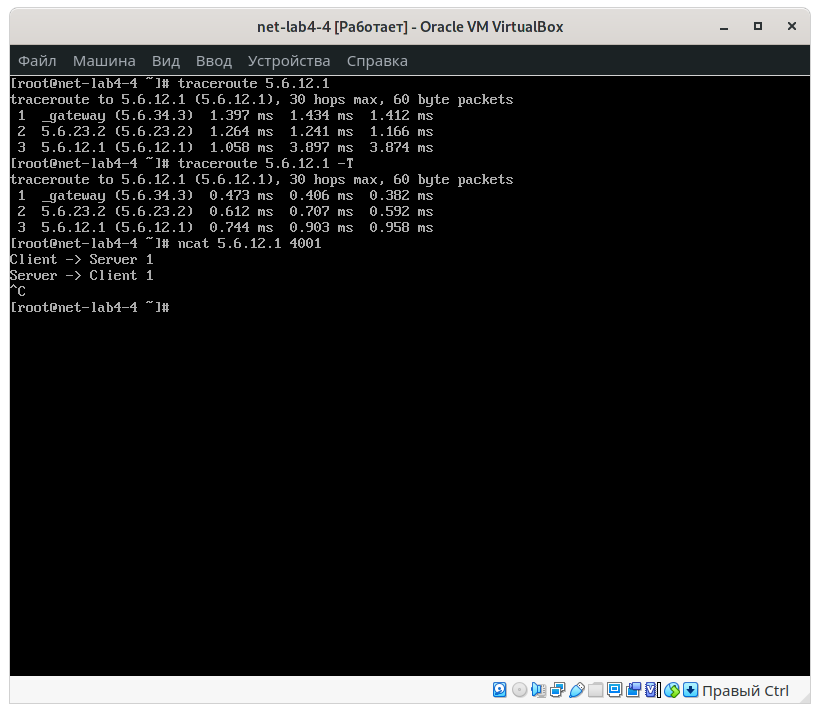
\includegraphics[width=.49\textwidth]{screenshots/var2-ncat1-client-ipv4}
\end{center}

\paragraph{IPv6}
\begin{center}
    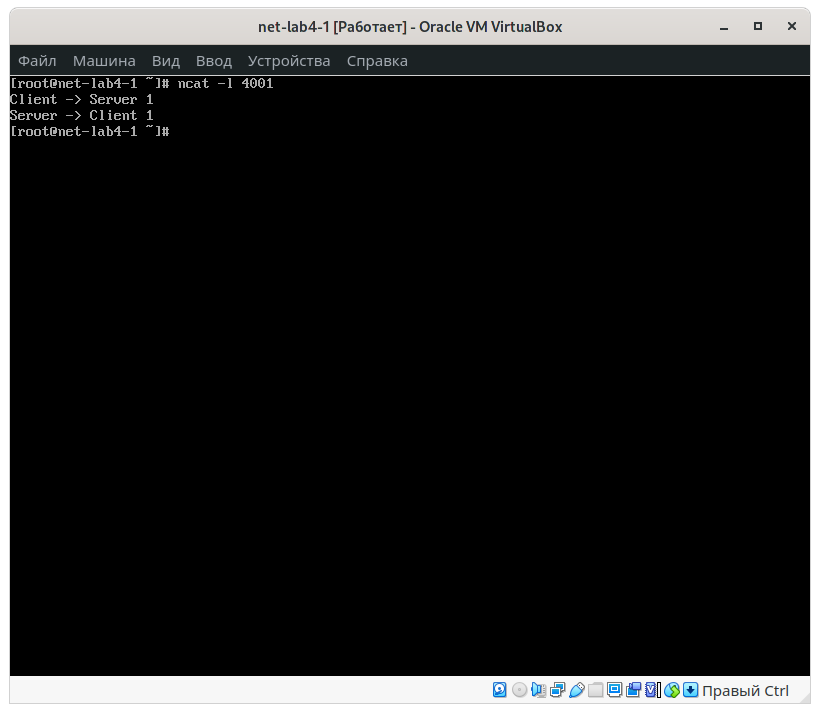
\includegraphics[width=.49\textwidth]{screenshots/var2-ncat1-server-ipv6}
    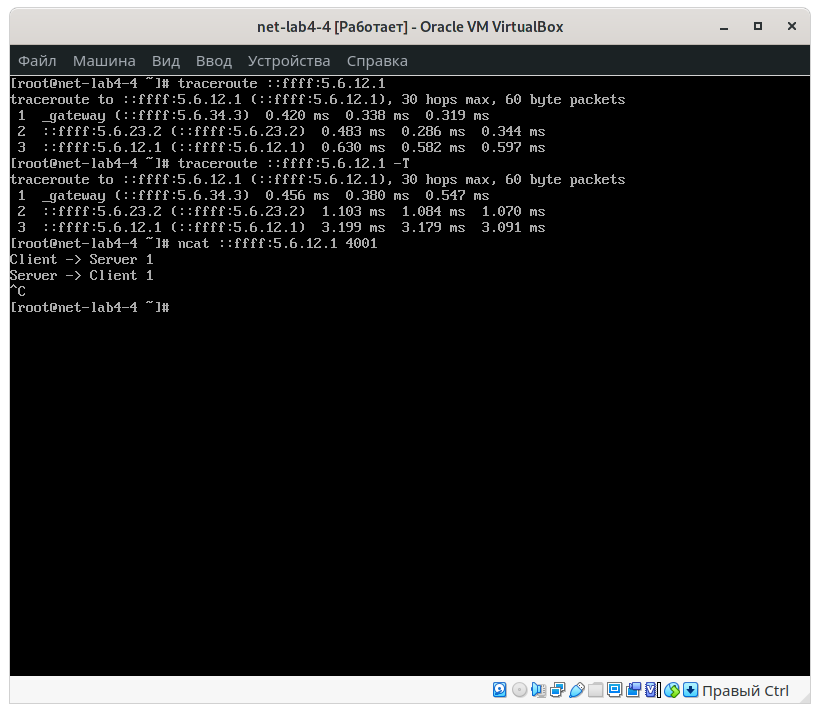
\includegraphics[width=.49\textwidth]{screenshots/var2-ncat1-client-ipv6}
\end{center}

\paragraph{\texttt{tcpdump}}
\begin{center}
    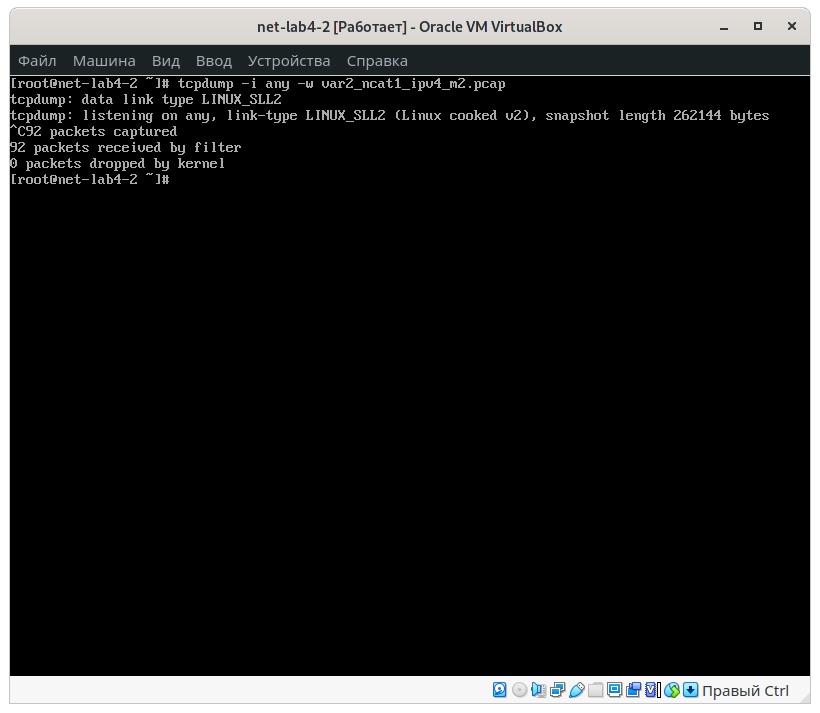
\includegraphics[width=.49\textwidth]{screenshots/var2-ncat1-ipv4-tcpdump2-1}
    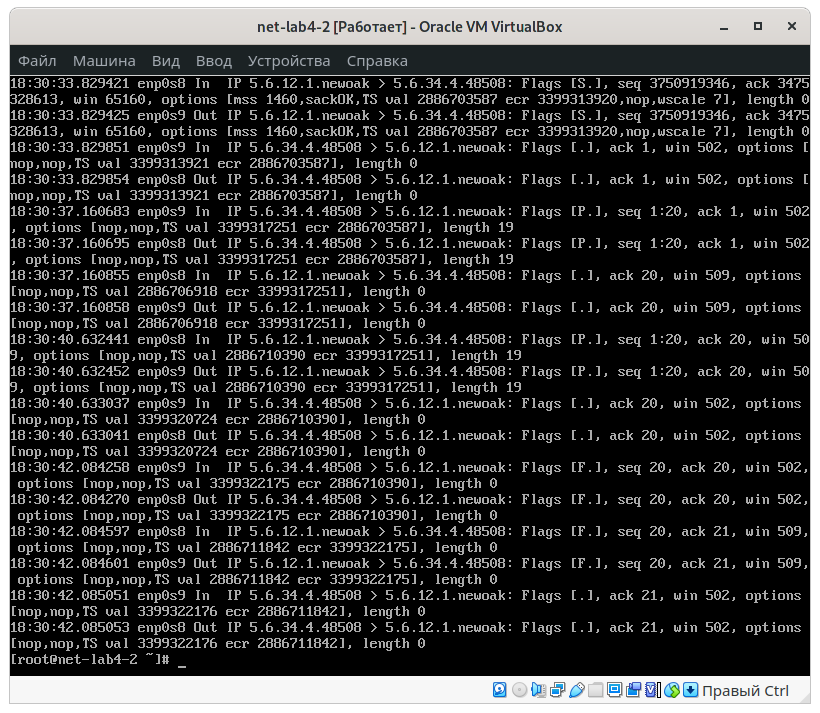
\includegraphics[width=.49\textwidth]{screenshots/var2-ncat1-ipv4-tcpdump2-2}

    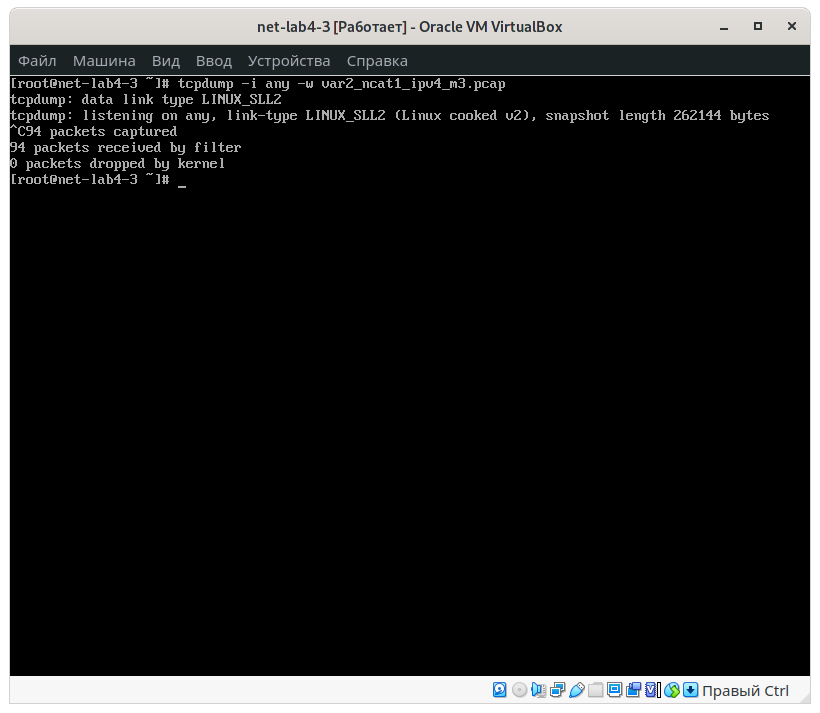
\includegraphics[width=.49\textwidth]{screenshots/var2-ncat1-ipv4-tcpdump3-1}
    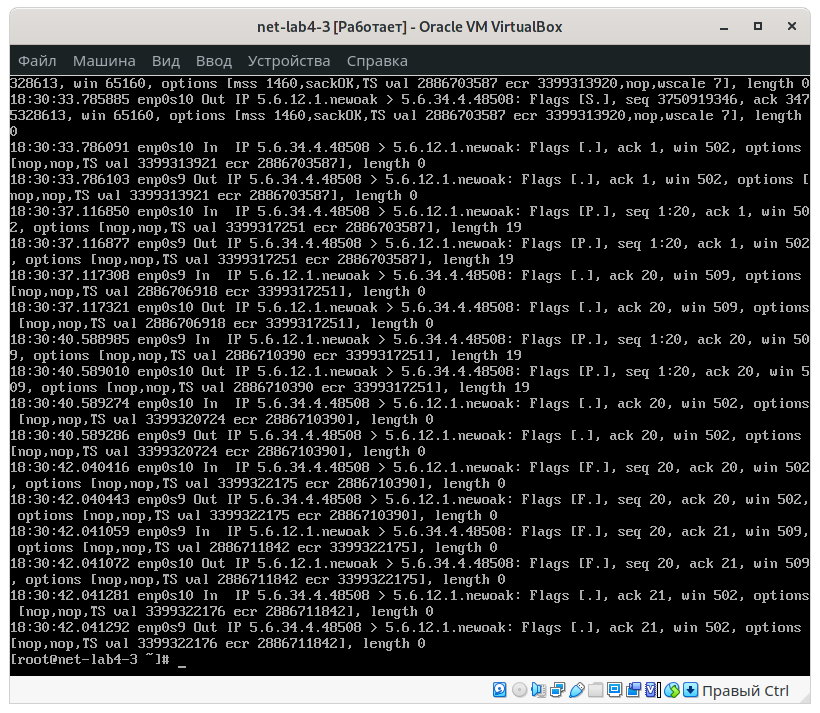
\includegraphics[width=.49\textwidth]{screenshots/var2-ncat1-ipv4-tcpdump3-2}

    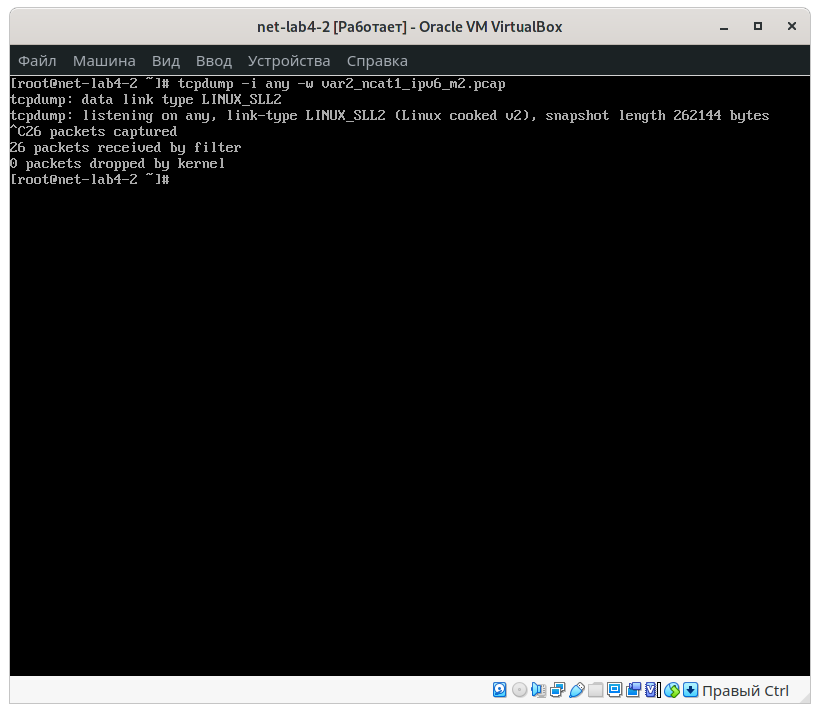
\includegraphics[width=.49\textwidth]{screenshots/var2-ncat1-ipv6-tcpdump2-1}
    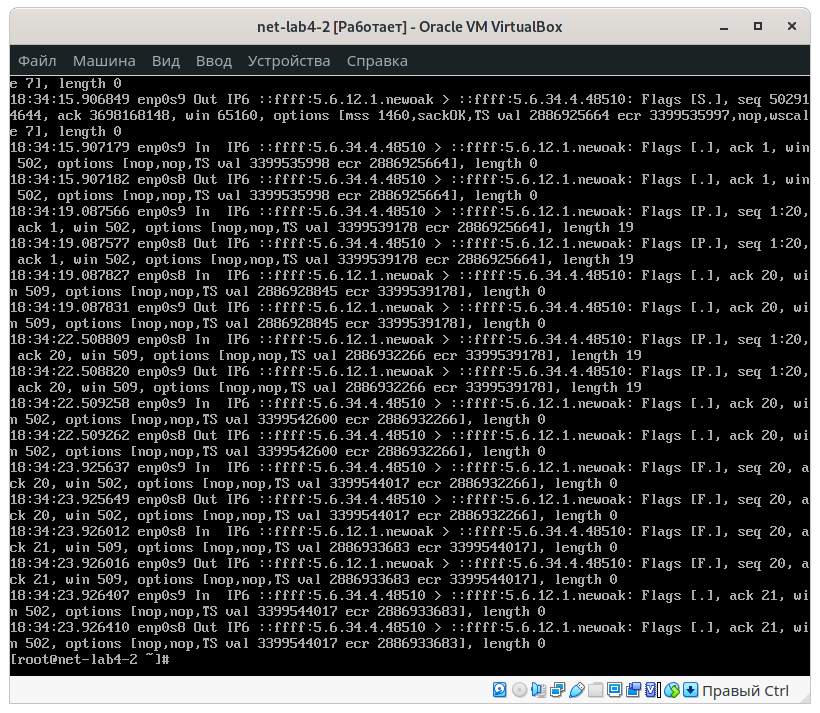
\includegraphics[width=.49\textwidth]{screenshots/var2-ncat1-ipv6-tcpdump2-2}

    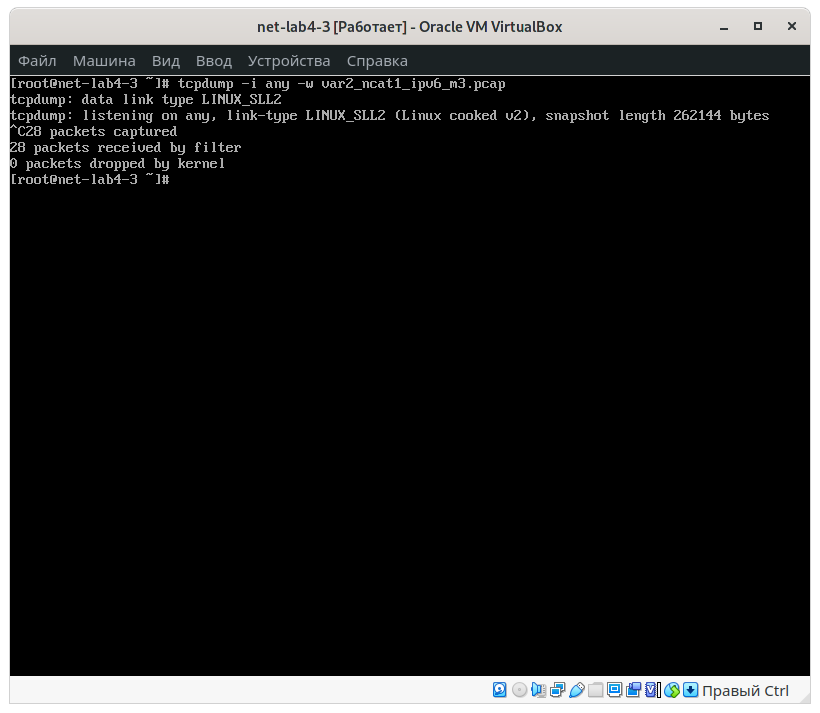
\includegraphics[width=.49\textwidth]{screenshots/var2-ncat1-ipv6-tcpdump3-1}
    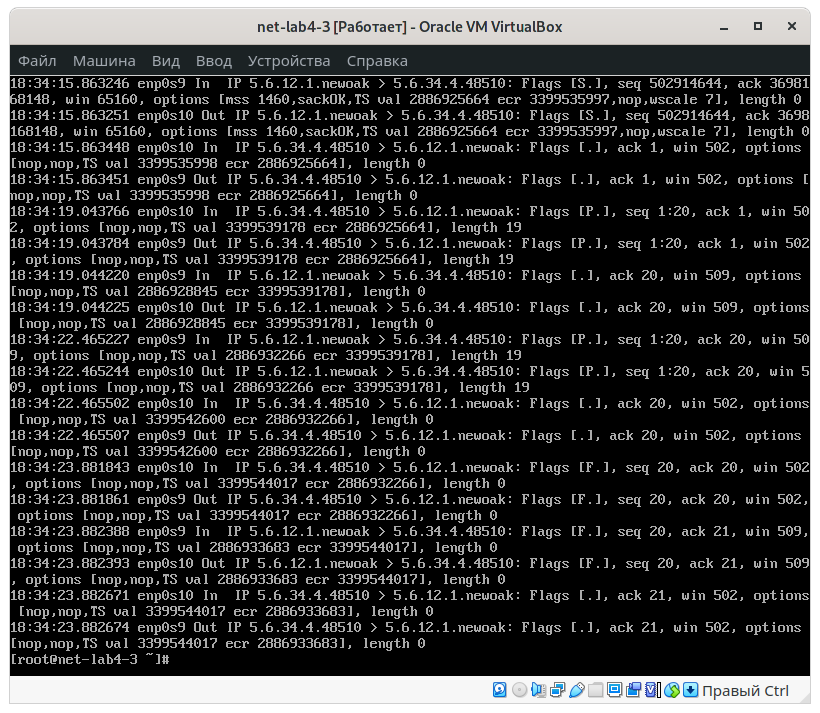
\includegraphics[width=.49\textwidth]{screenshots/var2-ncat1-ipv6-tcpdump3-2}
\end{center}

\subsubsection{Сервер 2}
\paragraph{IPv4}
\begin{center}
    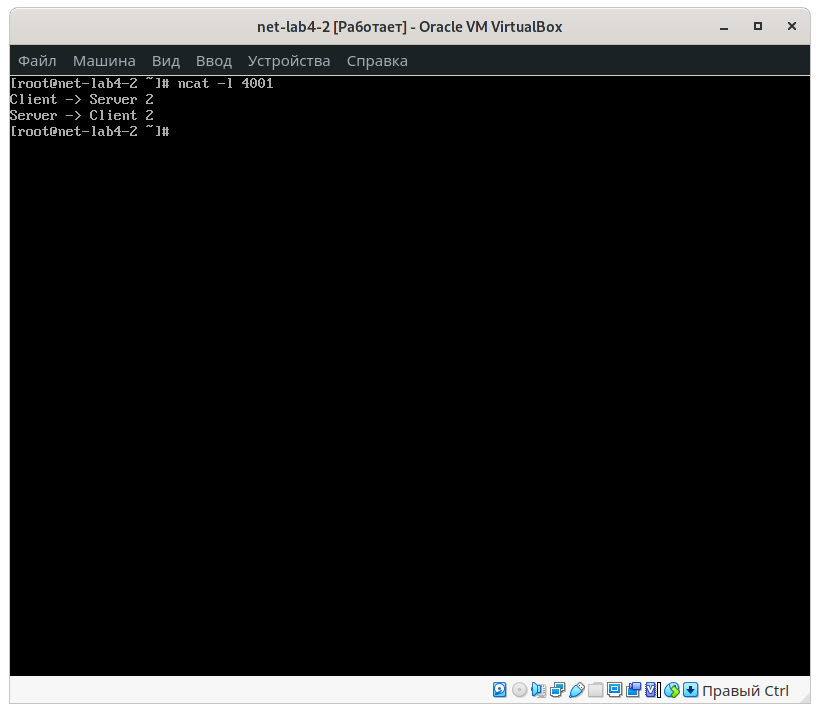
\includegraphics[width=.49\textwidth]{screenshots/var2-ncat2-server-ipv4}
    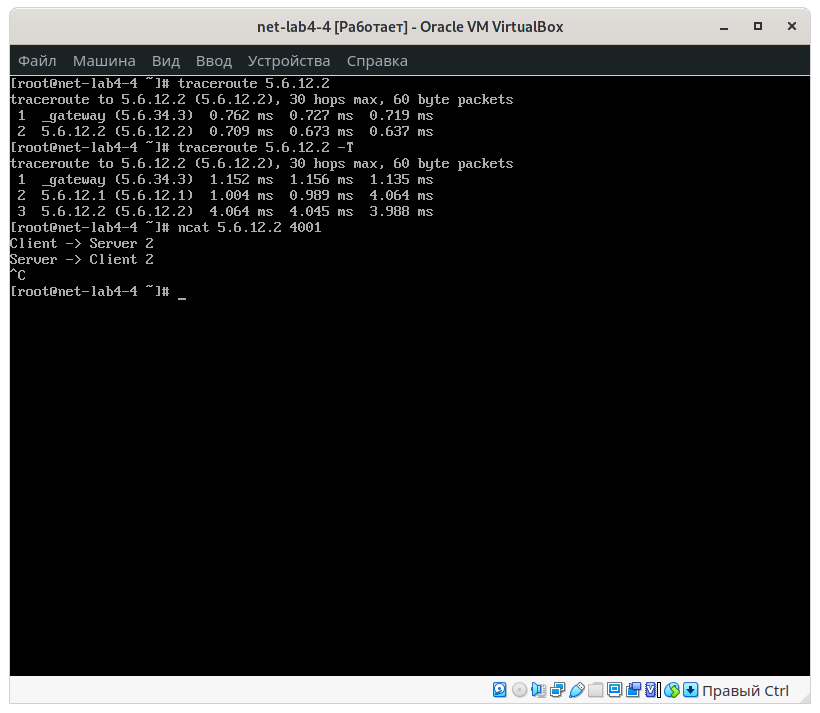
\includegraphics[width=.49\textwidth]{screenshots/var2-ncat2-client-ipv4}
\end{center}

\paragraph{IPv6}
\begin{center}
    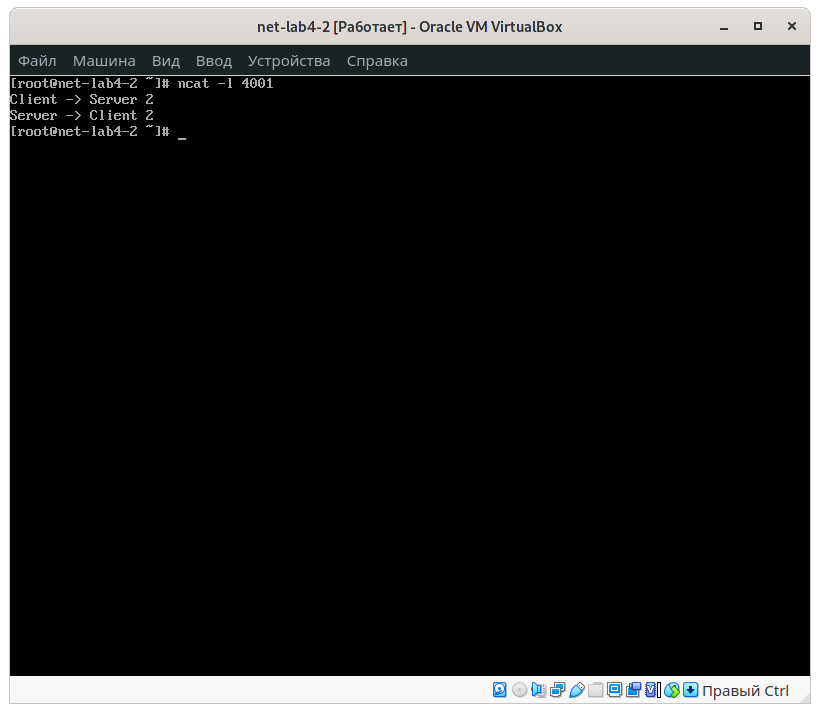
\includegraphics[width=.49\textwidth]{screenshots/var2-ncat2-server-ipv6}
    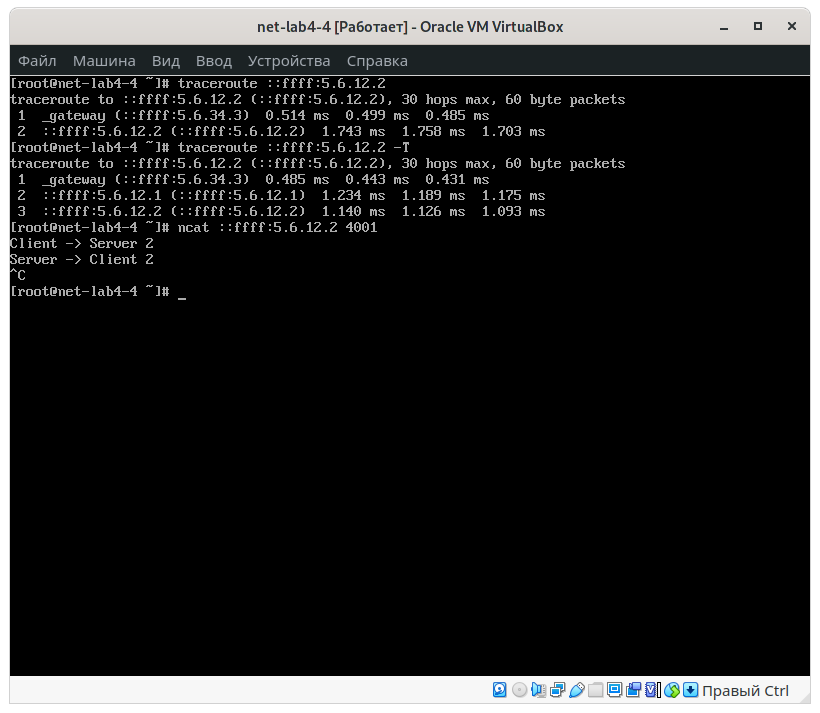
\includegraphics[width=.49\textwidth]{screenshots/var2-ncat2-client-ipv6}
\end{center}

\paragraph{\texttt{tcpdump}}
\begin{center}
    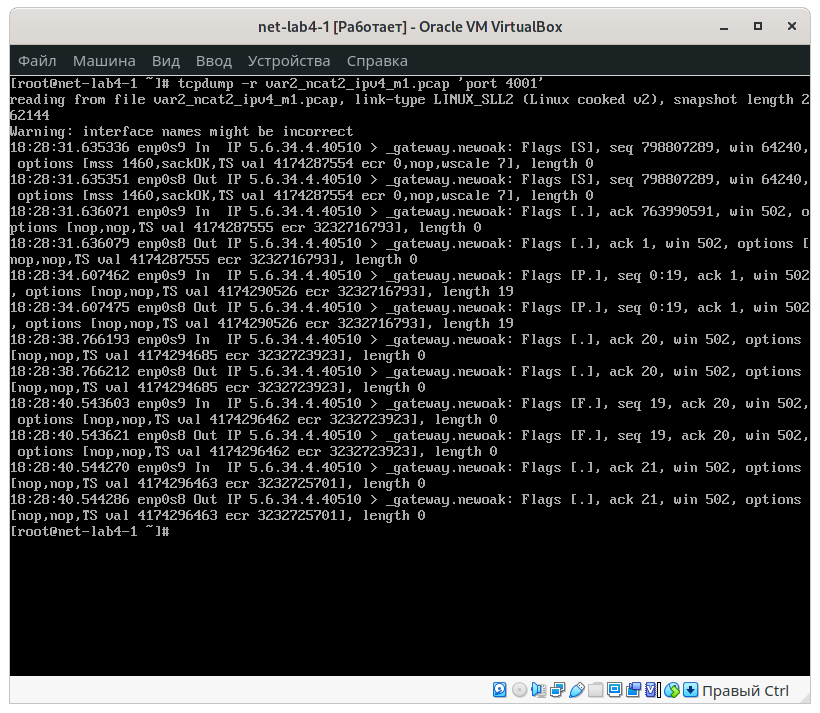
\includegraphics[width=.49\textwidth]{screenshots/var2-ncat2-ipv4-tcpdump1}
    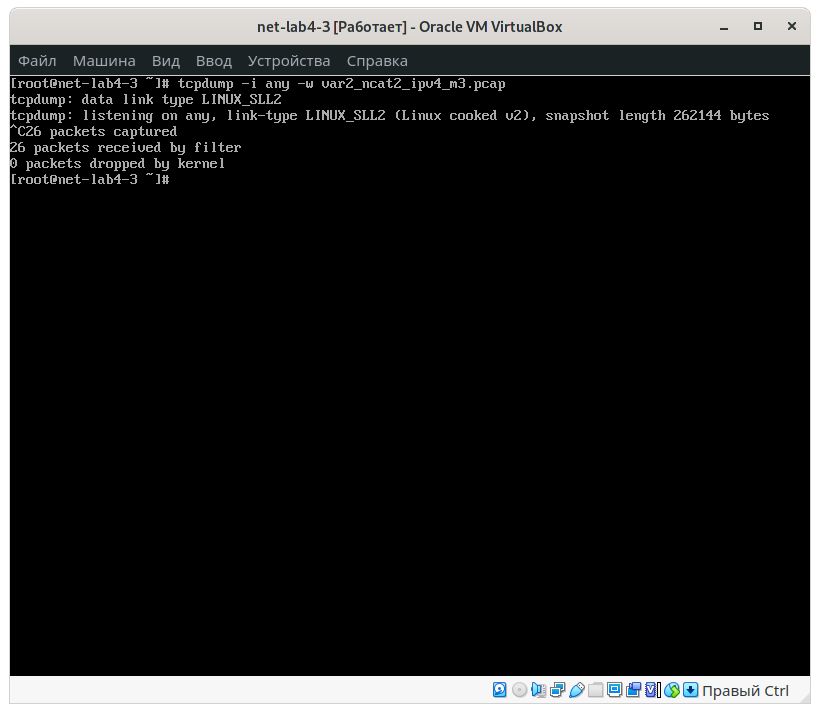
\includegraphics[width=.49\textwidth]{screenshots/var2-ncat2-ipv4-tcpdump3}
    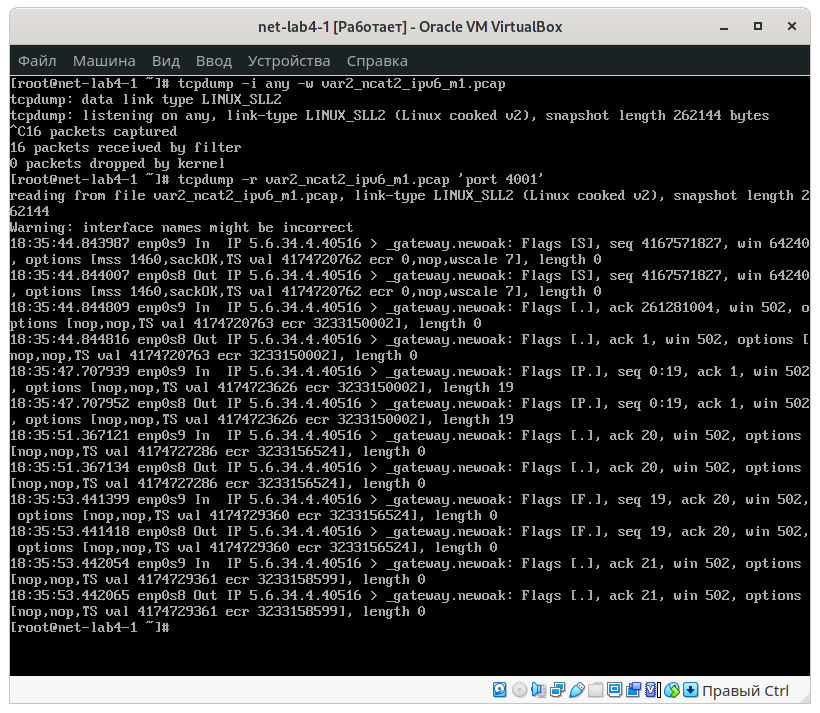
\includegraphics[width=.49\textwidth]{screenshots/var2-ncat2-ipv6-tcpdump1}

    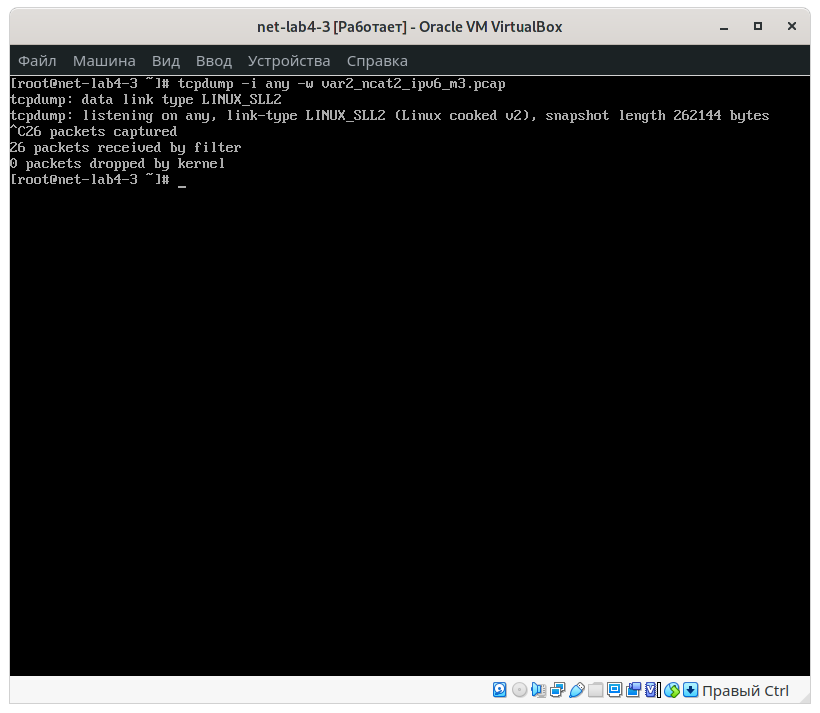
\includegraphics[width=.49\textwidth]{screenshots/var2-ncat2-ipv6-tcpdump3-1}
    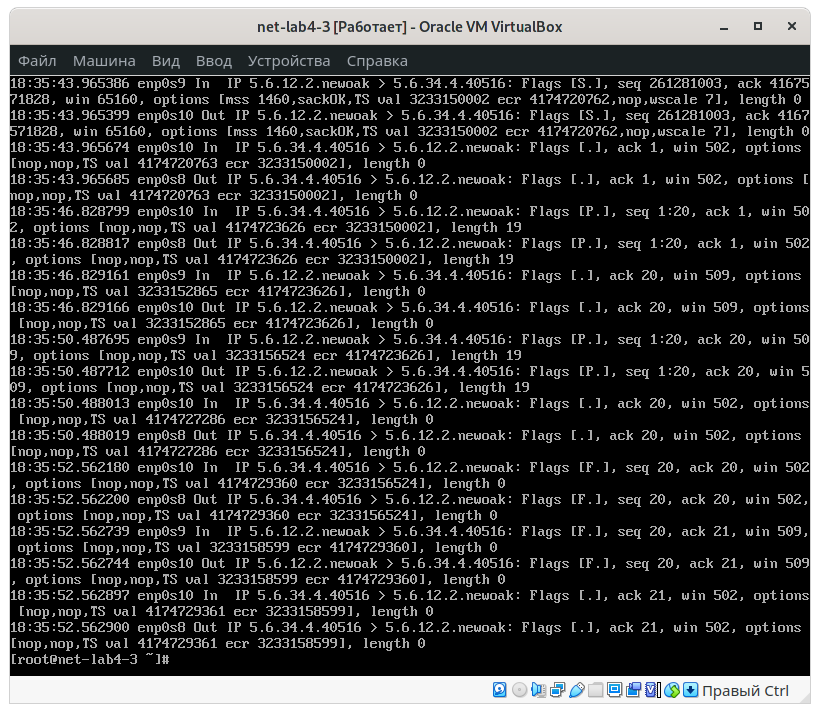
\includegraphics[width=.49\textwidth]{screenshots/var2-ncat2-ipv6-tcpdump3-2}
\end{center}
